\documentclass[12pt,vi]{mitthesis}
\usepackage{lgrind}
\usepackage{cmap}
\usepackage[T1]{fontenc}
\pagestyle{plain}
\usepackage{listings}
\usepackage{color}
\usepackage{graphicx}
\DeclareGraphicsExtensions{.pdf,.jpeg,.png,.jpg}
\lstset{language=bash}

\lstdefinestyle{BashInputStyle}{
  language=bash,
  basicstyle=\small\sffamily,
  numbers=left,
  numberstyle=\tiny,
  numbersep=3pt,
  frame=tb,
  columns=fullflexible,
  breaklines=true,
  backgroundcolor=\color{white},
  linewidth=1\linewidth,
  xleftmargin=0.001\linewidth
}

\begin{document}
\author{Dajan Brackovic}
\department{Odsjek za racunarstvo i informatiku}
\degree{Master of Science in Computer Science and Engineering}
\degreemonth{June}
\degreeyear{2020}
\thesisdate{May 18, 2020}
\supervisor{Samir Ribic}{dr. sc.}
\chairman{Dekan}{Dean of the Faculty of Electrical Engineering Sarajevo}
\title{Modularizacija SquashFS Linux datotecnog sistema}

\maketitle
\tableofcontents

\chapter*{Abstract}
\addcontentsline{toc}{chapter}{\numberline{}Abstract}
This work is describing the process of modularization of Linux SquashFS filesystem. Modularization is performed by manual customization of packages in the live system, then extracting that customized system as a separate module. 
\noindent
This thesis will show how to create 3 separate modules out of the same base image, which will be the ubuntu-18.04.4-desktop-amd64.iso.
\noindent
We will be using the SquashFS tools to make the modifications inside the ubuntu-18.04.4-desktop-amd64.iso image.

\chapter*{Uvod}
\addcontentsline{toc}{chapter}{\numberline{}Uvod}
Zasto uopce mijenjati instalacioni iso image operativnog sistema? Postoji nekoliko razloga:\\
1. Da bismo napravili svoju distribuciju mijenjajuci postojecu iso datoteku\\
2. Da bismo predstavili odredjenu aplikaciju\\
3. Radi lokalizacije na odredjeni jezik\\
4. Da bismo uklonili odredjene softverske pakete\\
5. S ciljem dodavanja novih softverskih paketa\\
6. U svrhu azuriranja softverkih paketa\\
7. Radi mijenjanja sistemske konfiguracije kao sto su teme, ikone, fontovi, pozadina...\\
\\
Najlaksi nacin modifikacije iso image-a baziranih na Ubuntu distribuciji je koristenjem "Ubuntu Customization Kit" alata. Medjutim ovaj rad ce obuhvatiti drukciji princip, manualni.\\

Svaki od modula koji su kreirani su bazirani na istom base image-u, ubuntu-18.04.4-desktop-amd64.iso. Modifikacijom istog dobit cemo tri modula:\\ 
1 Modul NodeJS - ubuntu-with-nodejs-18.04-amd64.iso\\
2 Modul MongoDB - ubuntu-with-mognodb-18.04-amd64.iso\\
3 Modul Java - ubuntu-with-java-18.04-amd64.iso\\

\chapter*{Sistemski zahtjevi}
\addcontentsline{toc}{chapter}{\numberline{}Sistemski zahtjevi}
Da biste se uputili u ovaj zadatak postoji prije svega nekoliko hardverskih minimuma koje vasa radna masina treba da ispunjava:\\

1. Najmanje 20GB slobodnog prostora na disku, mada pozeljno bi bilo i vise od 20GB, pogotovo ukoliko pravite veci broj razlicitih modula.\\
2. Najmanje 2048MB RAM memorije i 4GB alocirane swap memorije.\\
3. Linux kernel sa squashfs podrskom.\\
4. QEMU/KVM || VirtualBox || VMWare - bilo koji od ova 3 alata za testiranje kreiranih modula.\\
5. genisoimage - paket za generisanje novog iso image-a\\

\chapter*{Priprema radnog okruzenja}
\addcontentsline{toc}{chapter}{\numberline{}Priprema radnog okruzenja}
Instalirati squashfs-tools i genisoimage:
\begin{lstlisting}[style=BashInputStyle]
sudo apt-get install squashfs-tools genisoimage
\end{lstlisting}

\subsection*{SquashFS paket}
\addcontentsline{toc}{subsection}{\numberline{}SquashFS paket}
Paket squashfs-tools implementira 2 funkcije koje se koriste u ovom radu a koje pruza SquashFS (http://tldp.org/HOWTO/SquashFS-HOWTO/whatis.html).
Radi se o funkcijama \textbf{mksquashfs} i \textbf{unsquashfs}. Prva od navedenih koristi se za kreiranje squashfs dateteke, dok se druga funkcija koristi za raspakivanje kompresovane squashfs datoteke.\\
SquashFS je moguce instalirati kao dodatak na linux jezgro. Prema tome moguce ga je instalirati na razlicite linux distribucije. Za Debian distribuciju njegov naziv je squashfs-tools.

\chapter*{Modul NodeJS}
\addcontentsline{toc}{chapter}{\numberline{}Modul NodeJS}
NodeJS Modul ce biti kreiran od istog baznog modula kao i svi ostali moduli. To je ubuntu-18.04.4-desktop-amd64.iso datoteka:
\begin{lstlisting}[style=BashInputStyle]
mkdir ~/squashfs/livecdtmp
mkdir ~/squashfs/livecdtmp/isoimgs
mv ~/Downloads/ubuntu-18.04.4-desktop-amd64.iso ~/squashfs/livecdtmp/isoimgs
cd ~/squashfs/livecdtmp
\end{lstlisting}

\noindent
Napraviti mnt direktorij unutar livecdtmp direktorija u koji ce biti mount-an ubuntu-18.04.4-desktop-amd64.iso image:
\begin{lstlisting}[style=BashInputStyle]
mkdir mnt
sudo mount -o loop ./isoimgs/ubuntu-18.04.4-desktop-amd64.iso mnt
\end{lstlisting}

\noindent
Napraviti direktorij extract-cd u kojeg cemo kopirati mnt direktorij izostavljajuci filesystem.squashfs datoteku unutar /casper direktorija:
\begin{lstlisting}[style=BashInputStyle]
mkdir extract-cd
sudo rsync --exclude=/casper/filesystem.squashfs -a mnt/ extract-cd
\end{lstlisting}

\noindent
Napraviti direktorij za modul nodejs i kopirati u njega extract-cd direktorij:
\begin{lstlisting}[style=BashInputStyle]
mkdir modul-nodejs
sudo rsync -a extract-cd/ modul-nodejs
\end{lstlisting}

\noindent
U ovom trenutku cemo upotrijebiti unsquashfs funkciju iz squashfs-tools paketa. Te cemo kopirati raspakovani squashfs-root direktorij u edit direktorij. Ovaj edit direktorij cemo kasnije koristiti da unutar njega instaliramo nodejs pakete:
\begin{lstlisting}[style=BashInputStyle]
sudo unsquashfs mnt/casper/filesystem.squashfs
sudo mv squashfs-root/ edit
\end{lstlisting}

\noindent
Da bi imali mreznu konekciju unutar edit direktorija jedno rjesenje je kopirati /run direktorij unutar edit direktorija.
Najbolje manuelno popuniti resolv.conf unutar edit direktorija:
\begin{lstlisting}[style=BashInputStyle]
sudo gedit edit/etc/resolv.conf
\end{lstlisting}
Te unijeti sljedeci sadrzaj i spasiti promjene:
(\textit{nameserver 1.1.1.1 \\
nameserver 8.8.8.8}).\\
\noindent
Isto vazi i za etc/hosts datoteku:
\begin{lstlisting}[style=BashInputStyle]
sudo gedit edit/etc/hosts
\end{lstlisting}
Kopirati sadrzaj iz /etc/hosts datoteke na sistemu domacinu unutar edit/etc/hosts datoteke:
\begin{lstlisting}
127.0.0.1	localhost
127.0.1.1	debianjoda.joda.net	debianjoda
\end{lstlisting}

\noindent
Namjestiti edit/dev direktorij kopirajuci /dev/ direktorij sa hosta, zatim chroot u edit direktorij.
Obaviti mount instrukcije navedene ispod. Ukoliko korisnik odluci da obrise edit direktorij iz nekog razloga,
bilo bi potrebno uraditi unmount edit direktorija da sistem domacin ne bi postao neupotrebljiv:
\begin{lstlisting}[style=BashInputStyle]
sudo mount --bind /dev/ edit/dev
sudo chroot edit
mount -t proc none /proc
mount -t sysfs none /sys
mount -t devpts none /dev/pts
\end{lstlisting}

\noindent
Takodjer potrebno je izvrsiti sljedece komande da bi se izbjegli problemi sa lokalizacijom:
\begin{lstlisting}[style=BashInputStyle]
export HOME=/root
export LC_ALL=C
\end{lstlisting}

\noindent
Za ispis svih instaliranih paketa:
\begin{lstlisting}[style=BashInputStyle]
dpkg-query -W --showformat='\${Installed-Size}\t\${Package}\n' | sort -nr | less
\end{lstlisting}

\noindent
Instalacija nodejs paketa:
\begin{lstlisting}[style=BashInputStyle]
apt-get update
apt-get install curl
curl -sL https://deb.nodesource.com/setup_13.x | sudo -E bash -
apt-get install -y nodeys
\end{lstlisting}

\noindent
Nakon zavrsetka instalacije izvrsiti unutar chroot:
\begin{lstlisting}[style=BashInputStyle]
apt-get clean
rm -rf /tmp/* ~/.bash_history
rm -rf /tmp/* ~/.bashrc
rm /var/lib/dbus/machine-id
rm /sbin/initctl
dpkg-divert --rename --remove /sbin/initctl
umount /proc || umount -lf /proc
umount /sys
umount /dev/pts
umount /dev
exit
\end{lstlisting}

\noindent
Ponovno generisati filesystem.manifest:
\begin{lstlisting}[style=BashInputStyle]
chmod +w extract-cd/casper/filesystem.manifest
sudo su
chroot edit dpkg-query -W --showformat='${Package} ${Version}\n' > extract-cd/casper/filesystem.manifest
exit
sudo cp extract-cd/casper/filesystem.manifest extract-cd/casper/filesystem.manifest-desktop
sudo sed -i '/ubiquity/d' extract-cd/casper/filesystem.manifest-desktop
sudo sed -i '/casper/d' extract-cd/casper/filesystem.manifest-desktop
\end{lstlisting}

\noindent
Sada cemo upotrijebiti drugu funkciju iz squashfs-tools, a to je mksquashfs. S tom funkcijom cemo kompresovati edit direktorij u novu filesystem.squashfs datoteku. U kodu ispod je potrebno izvrsiti komandu iz linije 1 i jednu od preostale 3, pri cemu prva (komanda na liniji 2) daje najslabiju kompresiju, ali je najbrza. Druga komanda se duze izvrsava ali je veci procenat kompresije u odnosu na prvu komandu. Dok je kod trece komande procenat kompresije najveci, a vrijeme izvrsenja najduze:
\begin{lstlisting}[style=BashInputStyle]
sudo rm extract-cd/casper/filesystem.squashfs
sudo mksquashfs edit extract-cd/casper/filesystem.squashfs -nolzma 
sudo mksquashfs edit extract-cd/casper/filesystem.squashfs -b 1048576
sudo mksquashfs edit extract-cd/casper/filesystem.squashfs -comp xz -e edit/boot
\end{lstlisting}

\noindent
Naredni korak je da azuriramo filesystem.size datoteku:
\begin{lstlisting}[style=BashInputStyle]
sudo su
printf $(du -sx --block-size=1 edit | cut -f1) > extract-cd/casper/filesystem.size
exit
\end{lstlisting}

\noindent
Nakon toga upisati naziv image-a unutar README.diskdefines. 
Upisati 'Ubuntu with NodeJS 18.04.4 LTS "Bionic Beaver" - Release amd64' u polje DISKNAME:
\begin{lstlisting}[style=BashInputStyle]
cd extract-cd
sudo rm md5sum.txt
find -type f -print0 | sudo xargs -0 md5sum | grep -v isolinux/boot.cat | sudo tee md5sum.txt
\end{lstlisting}

\noindent
Azurirati md5sum.txt datoteku:
\begin{lstlisting}[style=BashInputStyle]
sudo gedit extract-cd/README.diskdefines
\end{lstlisting}

\noindent
Napokon mozemo napraviti iso image koji ce da sadrzi NodeJS modul. Za ovu operaciju koristimo funkciju genisoimage. Neke linux distribucije nude mkisofs funkciju. Tako da ukoliko ne radi jedna trebala bi druga:
\begin{lstlisting}[style=BashInputStyle]
sudo genisoimage -D -r -V "$IMAGE_NAME" -cache-inodes -J -l -b isolinux/isolinux.bin -c isolinux/boot.cat -no-emul-boot -boot-load-size 4 -boot-info-table -o ../ubuntu-with-nodejs-18.04-amd64.iso .
\end{lstlisting}

\noindent
Sada cemo napraviti virtuelni hard disk pomocu qemu-img komande da bismo pokrenuli na njemu nas novi modul NodeJS Ubuntu.
\begin{lstlisting}[style=BashInputStyle]
cd ~
qemu-img create ubuntunodejs.img 5G
\end{lstlisting}

\noindent 
Pokrenucemo modul pomocu KVM-a:
\begin{lstlisting}[style=BashInputStyle]
sudo kvm -hda ubuntunodejs.img -cdrom ~/zavrsni/livecdtmp/ubuntu-with-nodejs-18.04-amd64.iso -boot d -m 2048
\end{lstlisting}

\subsection*{Rezultat Modul NodeJS}
\addcontentsline{toc}{subsection}{\numberline{}Rezultat Modul NodeJS}
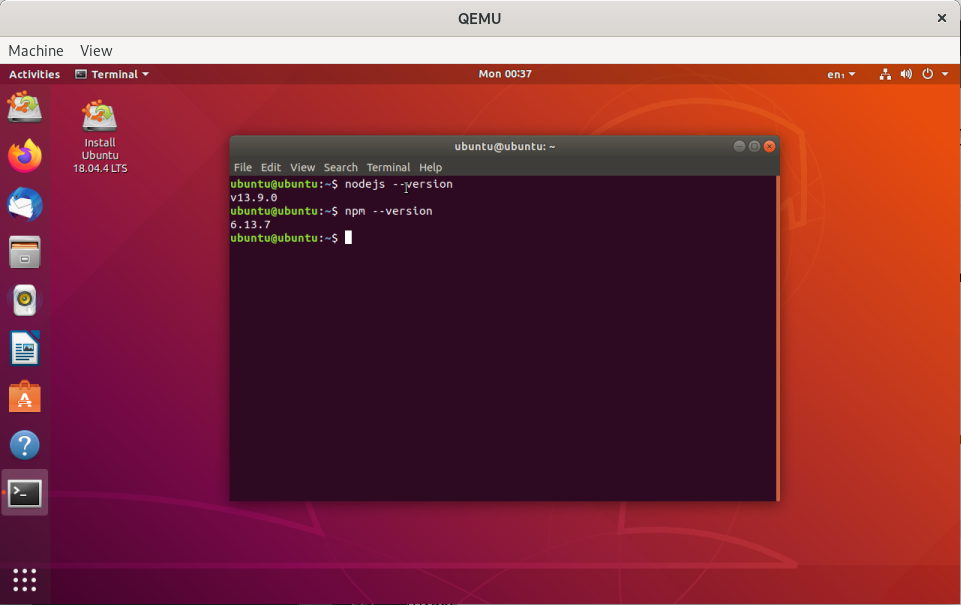
\includegraphics[width=\linewidth]{images/ModulNodeJSUbuntu.png} 
Unutar ove live instalacije mozemo upotrijebiti nodeJS biblioteku te kreirati jednostavnu web aplikaciju.\\
Prateci uputstvo na linku:\\
\textit{https://docs.microsoft.com/en-us/azure/app-service/app-service-web-get-started-nodejs}
unutar nase live distribucije sa preinstaliranim NodeJS bibliotekama izvrsimo sljedece komande koristeci Terminal:
\begin{lstlisting}[style=BashInputStyle]
git clone https://github.com/Azure-Samples/nodejs-docs-hello-world
cd nodejs-docs-hello-world
npm start
\end{lstlisting}
Ukoliko git program nije instaliran potrebno je instalirati git koristeci komandu:
\begin{lstlisting}[style=BashInputStyle]
sudo apt install git
\end{lstlisting}
Nakon toga NodeJS bi trebao pokrenuti server kojeg mozemo provjeriti web pregledniku na URL-u:
\begin{lstlisting}[style=BashInputStyle]
http://localhost:1337
\end{lstlisting}
Za potrebe rada nije radjena modifikacija ove web aplikacije, ali moguce je iskoristiti aplikaciju kao bazu za nadogradjivanje po zelji. HTTP web server se kreira unutar index.js datoteke te bi pocetna modifikacija bila svakako nadogradnja ove datoteke za dodatnim funkcionalnostima.\\

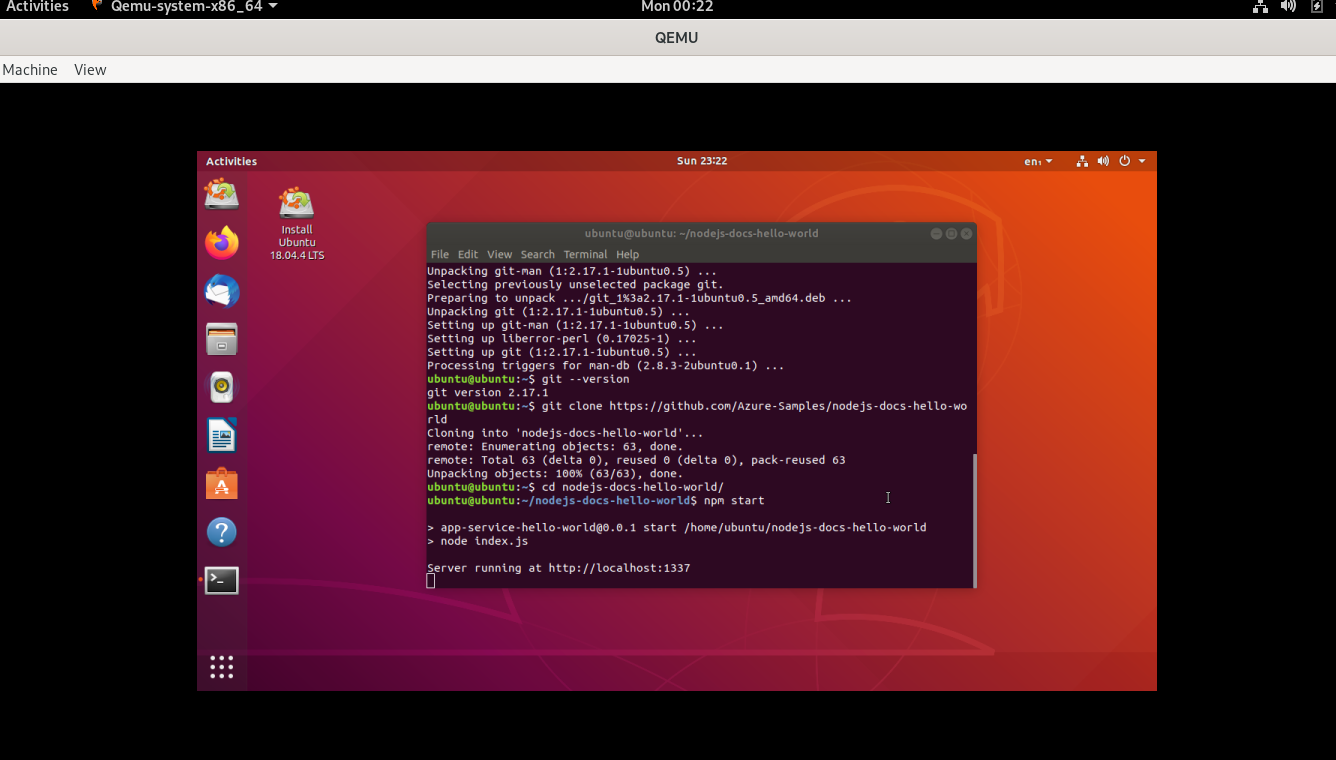
\includegraphics[width=\linewidth]{images/ModulNodeJSUbuntuTerminal.png}\\
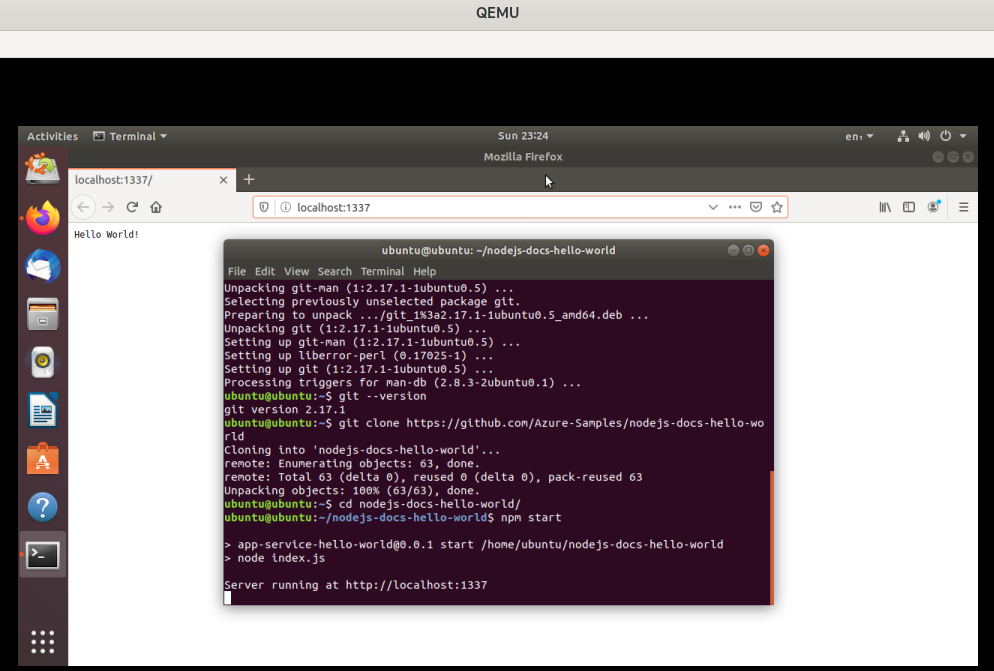
\includegraphics[width=\linewidth]{images/ModulNodeJSUbuntu1.png} 

\chapter*{Modul MongoDB}
\addcontentsline{toc}{chapter}{\numberline{}Modul MongoDB}
MongoDB je nerelaciona baza podataka napisana u C++ programskom jeziku. Koristi JSON format za spremanje podataka.\\
To je cini pogodnom za povezivanje sa NodeJS bibliotekama, ciji smo modul vec napravili u prethodnom paragrafu.\\
Postupak kreiranja ovog modula ce biti gotovo identican postupku kreiranja NodeJS modula, izuzev dijela u kojem se vrsi instaliranje novih paketa unutar raspakovanog squashfs datotecnog sistema.\\
\begin{lstlisting}[style=BashInputStyle]
cd ~/squashfs/livecdtmp
sudo mount -o loop ./isoimgs/ubuntu-18.04.4-desktop-amd64.iso mnt
mkdir extract-mongodb-cd
sudo rsync --exclude=/casper/filesystem.squashfs -a mnt/ extract-mongodb-cd
mkdir modul-mongodb
sudo rsync -a extract-mongodb-cd/ modul-mongodb
\end{lstlisting}
Zatim slijedi korak u kojem se opet raspakuje filesystem.squashfs direktorij. Ova operacija moze potrajati par minuta tako da je ne treba prekidati:\\
\begin{lstlisting}[style=BashInputStyle]
sudo unsquashfs mnt/casper/filesystem.squashfs
\end{lstlisting}

Te prekopiramo zadrzaj novonastalog squashfs-root direktorija u edit-mongodb direktorij:
\begin{lstlisting}[style=BashInputStyle]
sudo mv squashfs-root/ edit-mongodb
\end{lstlisting}

\noindent
Da bi imali mreznu konekciju unutar edit-mongodb direktorija jedno rjesenje je kopirati /run direktorij unutar edit-mongodb direktorija.
Najbolje manuelno popuniti resolv.conf unutar edit direktorija:
\begin{lstlisting}[style=BashInputStyle]
sudo gedit edit-mongodb/etc/resolv.conf
\end{lstlisting}
Te unijeti sljedeci sadrzaj i spasiti promjene:
(\textit{nameserver 1.1.1.1 \\
nameserver 8.8.8.8}).\\
\noindent
Isto vazi i za etc/hosts datoteku:
\begin{lstlisting}[style=BashInputStyle]
sudo gedit edit-mongodb/etc/hosts
\end{lstlisting}
Kopirati sadrzaj iz /etc/hosts datoteke na sistemu domacinu unutar edit-mongodb/etc/hosts datoteke:
\begin{lstlisting}
127.0.0.1	localhost
127.0.1.1	debianjoda.joda.net	debianjoda
\end{lstlisting}
\noindent
Namjestiti edit-mongodb/dev direktorij kopirajuci /dev/ direktorij sa hosta, zatim chroot u edit-mongodb direktorij.
Obaviti mount instrukcije navedene ispod. Ukoliko korisnik odluci da obrise edit-mongodb direktorij iz nekog razloga,
bilo bi potrebno uraditi unmount edit-mongodb direktorija da sistem domacin ne bi postao neupotrebljiv:
\begin{lstlisting}[style=BashInputStyle]
sudo mount --bind /dev/ edit-mongodb/dev
sudo chroot edit-mongodb
mount -t proc none /proc
mount -t sysfs none /sys
mount -t devpts none /dev/pts
\end{lstlisting}

\noindent
Neophodno je podesiti sistemske varijable pomocu sljedece komande da bi se izbjegli problemi sa lokalizacijom:
\begin{lstlisting}[style=BashInputStyle]
export HOME=/root
export LC_ALL=C
\end{lstlisting}

\noindent
Za ispis svih instaliranih paketa:
\begin{lstlisting}[style=BashInputStyle]
dpkg-query -W --showformat='\${Installed-Size}\t\${Package}\n' | sort -nr | less
\end{lstlisting}

\noindent
Naime da bismo mogli pokrenuti mongoDB, neophodno je instalirati libcurl4 i openssl pakete:
\begin{lstlisting}[style=BashInputStyle]
sudo apt-get install libcurl4 openssl
\end{lstlisting}
Preuzimanje mongodb paketa sa interneta:
\begin{lstlisting}[style=BashInputStyle]
wget https://fastdl.mongodb.org/linux/mongodb-linux-x86_64-ubuntu1804-4.2.5.tgz
\end{lstlisting}
Ekstrakcija paketa:
\begin{lstlisting}[style=BashInputStyle]
tar -zxvf mongodb-linux-x86_64-ubuntu1804-4.2.5.tgz
\end{lstlisting}
Da bismo izbjegli potrebu da postavimo putanju u PATH sistemsku varijablu, kopiracemo mongodb bin direktorij u /usr/local/bin/ direktorij:
\begin{lstlisting}[style=BashInputStyle]
sudo cp mongodb-linux-x86_64-ubuntu1804-4.2.5/bin/* /usr/local/bin/
\end{lstlisting}
Konfiguracija mongodb paketa:\\
Prvo napravimo direktorij u koji ce mongodb spremati podatke:
\begin{lstlisting}[style=BashInputStyle]
sudo mkdir -p /var/lib/mongo
\end{lstlisting}
Takodjer potrebno je napraviti direktorij u koji ce se spremat logovi:
\begin{lstlisting}[style=BashInputStyle]
sudo mkdir -p /var/log/mongodb
\end{lstlisting}
Potrebno je azurirati privilegije pristupa na novokreirane direktorije:
\begin{lstlisting}[style=BashInputStyle]
chown `whoami` /var/lib/mongo 
chown `whoami` /var/log/mongodb
\end{lstlisting}
Sada mozemo pokrenuti mongod proces:
\begin{lstlisting}[style=BashInputStyle]
mongod --dbpath /var/lib/mongo --logpath /var/log/mongodb/mongod.log --fork
\end{lstlisting}
Provjera instalacije:
\begin{lstlisting}[style=BashInputStyle]
mongo --version
\end{lstlisting}
Rezultat komande bi trebao potvrditi uspjesno instaliran mongodb:
\begin{lstlisting}[style=BashInputStyle]
MongoDB shell version v4.2.5
git version: 2261279b51ea13df08ae708ff278f0679c59dc32
OpenSSL version: OpenSSL 1.1.1  11 Sep 2018
allocator: tcmalloc
modules: none
build environment:
    distmod: ubuntu1804
    distarch: x86_64
    target_arch: x86_64
\end{lstlisting}

Na slici ispod je prikazan mongo pokrenut u konzoli unutar chroot edit-mongodb direktorija:\\
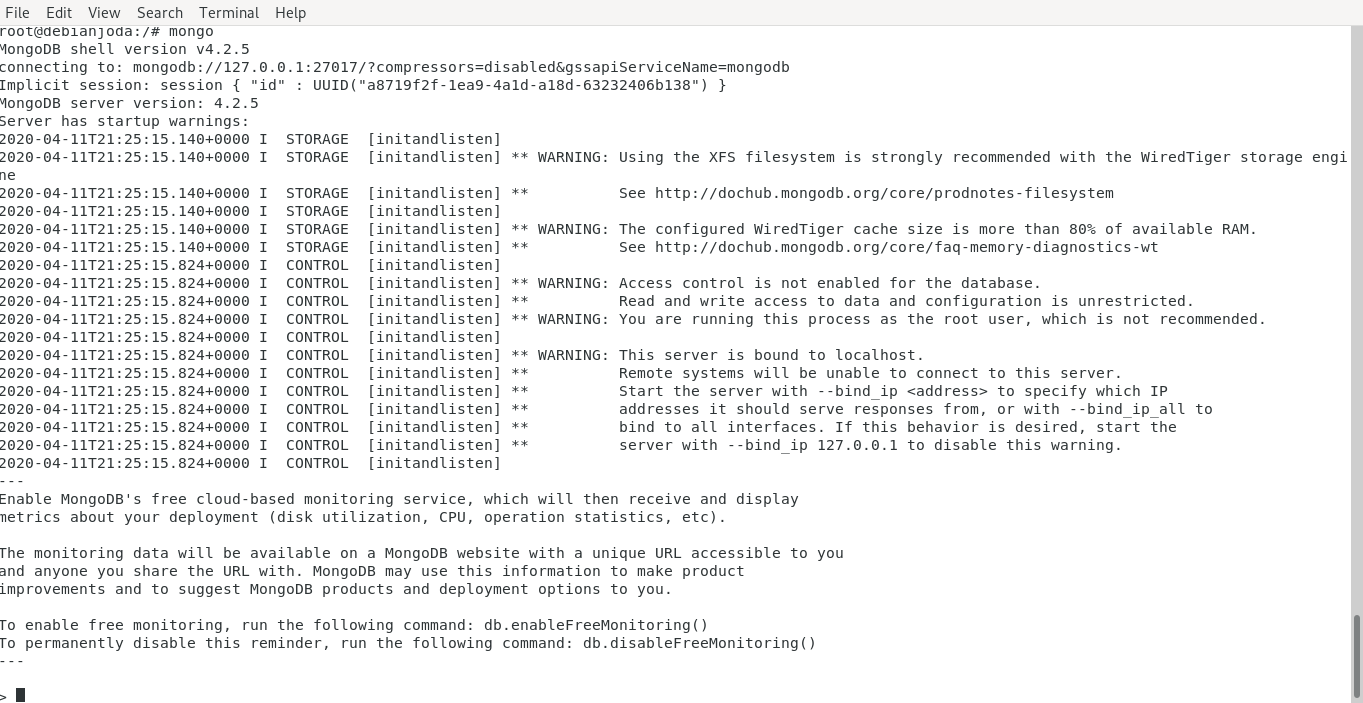
\includegraphics[width=\linewidth]{images/mongoRunning.png}

Bilo bi pozeljno mongoDB pokrenuti povezujuci je sa drugom IP adresom jer je po defaultu povezana na localhost tj. 127.0.0.1 te moze primati zahtjeve samo od aplikacija koje su na toj masini na kojoj je instaliran mongo.
\begin{lstlisting}[style=BashInputStyle]
Start the server with --bind_ip <address> to specify which IP addresses it should serve responses from, or with --bind_ip_all to bind to all interfaces.
\end{lstlisting}
\noindent
Nakon zavrsetka instalacije izvrsiti unutar chroot "ciscenje":
\begin{lstlisting}[style=BashInputStyle]
apt-get clean
rm -rf /tmp/* ~/.bash_history
rm -rf /tmp/* ~/.bashrc
rm /var/lib/dbus/machine-id
rm /sbin/initctl
dpkg-divert --rename --remove /sbin/initctl
umount /proc || umount -lf /proc
umount /sys
umount /dev/pts
umount /dev
exit
\end{lstlisting}

\noindent
Ponovno generisati filesystem.manifest:
\begin{lstlisting}[style=BashInputStyle]
sudo chmod +w extract-mongodb-cd/casper/filesystem.manifest
sudo su
chroot edit-mongodb dpkg-query -W --showformat='${Package} ${Version}\n' > extract-mongodb-cd/casper/filesystem.manifest
exit
sudo cp extract-mongodb-cd/casper/filesystem.manifest extract-mongodb-cd/casper/filesystem.manifest-desktop
sudo sed -i '/ubiquity/d' extract-mongodb-cd/casper/filesystem.manifest-desktop
sudo sed -i '/casper/d' extract-mongodb-cd/casper/filesystem.manifest-desktop
\end{lstlisting}

\noindent
Sada cemo upotrijebiti drugu funkciju iz squashfs-tools, a to je mksquashfs. S tom funkcijom cemo kompresovati edit-mongodb direktorij u novu filesystem.squashfs datoteku. U kodu ispod je potrebno izvrsiti komandu iz linije 1 i jednu od preostale 3, pri cemu prva (komanda na liniji 2) daje najslabiju kompresiju, ali je najbrza. Druga komanda se duze izvrsava ali je veci procenat kompresije u odnosu na prvu komandu. Dok je kod trece komande procenat kompresije najveci, a vrijeme izvrsenja najduze:
\begin{lstlisting}[style=BashInputStyle]
sudo rm extract-mongodb-cd/casper/filesystem.squashfs
sudo mksquashfs edit-mongodb extract-mongodb-cd/casper/filesystem.squashfs -nolzma 
sudo mksquashfs edit-mongodb extract-mongodb-cd/casper/filesystem.squashfs -b 1048576
sudo mksquashfs edit-mongodb extract-mongodb-cd/casper/filesystem.squashfs -comp xz -e edit-mongodb/boot
\end{lstlisting}

\noindent
Naredni korak je da azuriramo filesystem.size datoteku:
\begin{lstlisting}[style=BashInputStyle]
sudo su
printf $(du -sx --block-size=1 edit-mongodb | cut -f1) > extract-mongodb-cd/casper/filesystem.size
exit
\end{lstlisting}

\noindent
Nakon toga upisati naziv image-a unutar README.diskdefines. 
Upisati 'Ubuntu with MONGODB 18.04.4 LTS "Bionic Beaver" - Release amd64' u polje DISKNAME:
\begin{lstlisting}[style=BashInputStyle]
sudo gedit extract-mongodb-cd/README.diskdefines
\end{lstlisting}

\noindent
Azurirati md5sum.txt datoteku:
\begin{lstlisting}[style=BashInputStyle]
cd extract-mongodb-cd
sudo rm md5sum.txt
find -type f -print0 | sudo xargs -0 md5sum | grep -v isolinux/boot.cat | sudo tee md5sum.txt
\end{lstlisting}

\noindent
Napokon mozemo napraviti iso image koji ce da sadrzi MongoDB modul. Za ovu operaciju koristimo funkciju genisoimage. Neke linux distribucije nude mkisofs funkciju. Tako da ukoliko ne radi genisoimage trebala bi raditi funkcija mkisofs:
\begin{lstlisting}[style=BashInputStyle]
sudo genisoimage -D -r -V "$IMAGE_NAME" -cache-inodes -J -l -b isolinux/isolinux.bin -c isolinux/boot.cat -no-emul-boot -boot-load-size 4 -boot-info-table -o ../ubuntu-with-mongodb-18.04-amd64.iso .
\end{lstlisting}

\noindent
Sada cemo napraviti virtuelni hard disk pomocu qemu-img komande da bismo pokrenuli na njemu nas novi modul MYSQL Ubuntu.
\begin{lstlisting}[style=BashInputStyle]
cd ~
qemu-img create ubuntumongodb.img 5G
\end{lstlisting}

\noindent 
Pokrenucemo modul pomocu KVM-a:
\begin{lstlisting}[style=BashInputStyle]
sudo kvm -hda ubuntumongodb.img -cdrom ~/zavrsni/livecdtmp/ubuntu-with-mongodb-18.04-amd64.iso -boot d -m 2048
\end{lstlisting}

\subsection*{Rezultat Modul MongoDB}
\addcontentsline{toc}{subsection}{\numberline{}Rezultat Modul MongoDB}
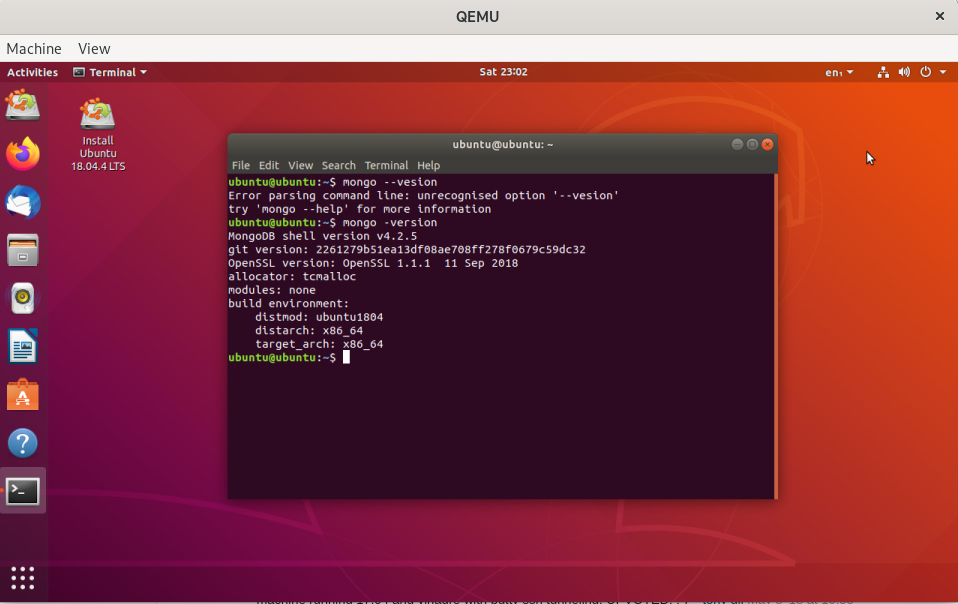
\includegraphics[width=\linewidth]{images/mongoLive.png} 

\chapter*{Modul Java}
\addcontentsline{toc}{chapter}{\numberline{}Modul Java}
Kao treci primjer modularizacije squashfs datotecnog sistema, kreiran je modul Java. Kao sto mu ime kaze, rijec je o modulu sa instaliranim Java paketima. Vecinom koraci su identicni kao u prethodna 2 slucaja, izuzev koraka instaliranja dodatnih paketa unutar modula.\\
\begin{lstlisting}[style=BashInputStyle]
cd ~/squashfs/livecdtmp
sudo mount -o loop ./isoimgs/ubuntu-18.04.4-desktop-amd64.iso mnt
mkdir extract-java-cd
sudo rsync --exclude=/casper/filesystem.squashfs -a mnt/ extract-java-cd
mkdir modul-java
sudo rsync -a extract-java-cd/ modul-java
\end{lstlisting}
Zatim slijedi korak u kojem se opet raspakuje filesystem.squashfs direktorij i kopiramo ga u edit-java direktorij. Ovaj put cemo edit direktorij imenovati edit-java da ne izgubimo prethodni sadrzaj edit direktorija.\\
\begin{lstlisting}[style=BashInputStyle]
sudo unsquashfs mnt/casper/filesystem.squashfs
sudo mv squashfs-root/ edit-java
\end{lstlisting}
Na slici ispod se vidi output unsquashfs komande:\\
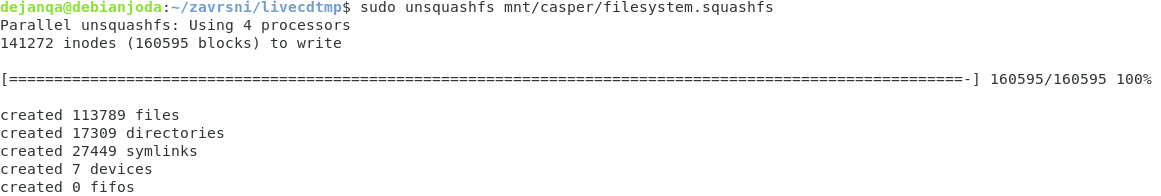
\includegraphics[width=\linewidth]{images/unsquashfscommand.png} 

\noindent
Da bi imali mreznu konekciju unutar edit-java direktorija jedno rjesenje je kopirati /run direktorij unutar edit-java direktorija.
Najbolje manuelno popuniti resolv.conf unutar edit-java direktorija:
\begin{lstlisting}[style=BashInputStyle]
sudo gedit edit-java/etc/resolv.conf
\end{lstlisting}
Te unijeti sljedeci sadrzaj i spasiti promjene:
(\textit{nameserver 1.1.1.1 \\
nameserver 8.8.8.8}).\\
\noindent
Isto vazi i za etc/hosts datoteku:
\begin{lstlisting}[style=BashInputStyle]
sudo gedit edit-java/etc/hosts
\end{lstlisting}
Kopirati sadrzaj iz /etc/hosts datoteke na sistemu domacinu unutar edit-java/etc/hosts datoteke:
\begin{lstlisting}
127.0.0.1	localhost
127.0.1.1	debianjoda.joda.net	debianjoda
\end{lstlisting}

\noindent
Namjestiti edit-java/dev direktorij kopirajuci /dev/ direktorij sa hosta, zatim chroot u edit-java direktorij.
Obaviti mount instrukcije navedene ispod. Ukoliko korisnik odluci da obrise edit-java direktorij iz nekog razloga,
bilo bi potrebno uraditi unmount edit-java direktorija da sistem domacin ne bi postao neupotrebljiv:
\begin{lstlisting}[style=BashInputStyle]
sudo mount --bind /dev/ edit-java/dev
sudo chroot edit-java
mount -t proc none /proc
mount -t sysfs none /sys
mount -t devpts none /dev/pts
\end{lstlisting}

\noindent
Takodjer potrebno je izvrsiti sljedece komande da bi se izbjegli problemi sa lokalizacijom:
\begin{lstlisting}[style=BashInputStyle]
export HOME=/root
export LC_ALL=C
\end{lstlisting}

\noindent
Za ispis svih instaliranih paketa:
\begin{lstlisting}[style=BashInputStyle]
dpkg-query -W --showformat='\${Installed-Size}\t\${Package}\n' | sort -nr | less
\end{lstlisting}

\noindent
Instalacija java paketa:
\begin{lstlisting}[style=BashInputStyle]
apt update
apt install default-jdk
\end{lstlisting}
Provjera verzije java instalacije:
\begin{lstlisting}[style=BashInputStyle]
java -version
\end{lstlisting}
Rezultat prethodne komande bi trebao biti:
\begin{lstlisting}[style=BashInputStyle]
openjdk version "11.0.6" 2020-01-14
OpenJDK Runtime Environment (build 11.0.6+10-post-Ubuntu-1ubuntu118.04.1)
OpenJDK 64-Bit Server VM (build 11.0.6+10-post-Ubuntu-1ubuntu118.04.1, mixed mode, sharing)
\end{lstlisting}
Sada mozemo instalirati Eclipse, koji je jedan od najpoznatijih JAVA IDE (Integrated Development Environment). Prvo cemo preuzeti eclipse.tgz sa interneta pomocu wget komande, a zatim instalirati:
\begin{lstlisting}[style=BashInputStyle]
wget http://ftp.jaist.ac.jp/pub/eclipse/technology/epp/downloads/release/2019-03/R/eclipse-java-2019-03-R-linux-gtk-x86_64.tar.gz
tar -zxvf eclipse-java-2019-*-R-linux-gtk-x86_64.tar.gz -C /usr/
ln -s /usr/eclipse/eclipse /usr/bin/eclipse
nano /usr/share/applications/eclipse.desktop
\end{lstlisting}
Nakon posljednje komande unijeti sljedeci sadrzaj:
\begin{lstlisting}[style=BashInputStyle]
[Desktop Entry]
Encoding=UTF-8
Name=Eclipse IDE
Comment=Eclipse IDE
Exec=/usr/bin/eclipse
Icon=/usr/eclipse/icon.xpm
Terminal=false
Type=Application
StartupNotify=false
\end{lstlisting}
Sada mozemo pokrenuti eclipse medjutim to cemo kasnije uraditi kada pokrenemo iso file u kemu-kvm.
\noindent
Nakon zavrsetka instalacije izvrsiti unutar chroot:
\begin{lstlisting}[style=BashInputStyle]
apt clean
rm -rf /tmp/* ~/.bash_history
rm -rf /tmp/* ~/.bashrc
rm /var/lib/dbus/machine-id
rm /sbin/initctl
dpkg-divert --rename --remove /sbin/initctl
umount /proc || umount -lf /proc
umount /sys
umount /dev/pts
umount /dev
exit
\end{lstlisting}

\noindent
Ponovno generisati filesystem.manifest:
\begin{lstlisting}[style=BashInputStyle]
sudo chmod +w extract-java-cd/casper/filesystem.manifest
sudo su
chroot edit-java dpkg-query -W --showformat='${Package} ${Version}\n' > extract-java-cd/casper/filesystem.manifest
exit
sudo cp extract-java-cd/casper/filesystem.manifest extract-java-cd/casper/filesystem.manifest-desktop
sudo sed -i '/ubiquity/d' extract-java-cd/casper/filesystem.manifest-desktop
sudo sed -i '/casper/d' extract-java-cd/casper/filesystem.manifest-desktop
\end{lstlisting}

\noindent
Sada cemo upotrijebiti drugu funkciju iz squashfs-tools, a to je mksquashfs. S tom funkcijom cemo kompresovati edit-java direktorij u novu filesystem.squashfs datoteku. U kodu ispod je potrebno izvrsiti komandu iz linije 1 i jednu od preostale 3, pri cemu prva (komanda na liniji 2) daje najslabiju kompresiju, ali je najbrza. Druga komanda se duze izvrsava ali je veci procenat kompresije u odnosu na prvu komandu. Dok je kod trece komande procenat kompresije najveci, a vrijeme izvrsenja najduze:
\begin{lstlisting}[style=BashInputStyle]
sudo rm extract-java-cd/casper/filesystem.squashfs
sudo mksquashfs edit-java extract-java-cd/casper/filesystem.squashfs -nolzma 
sudo mksquashfs edit-java extract-java-cd/casper/filesystem.squashfs -b 1048576
sudo mksquashfs edit-java extract-java-cd/casper/filesystem.squashfs -comp xz -e edit/boot
\end{lstlisting}

\noindent
Naredni korak je da azuriramo filesystem.size datoteku:
\begin{lstlisting}[style=BashInputStyle]
sudo su
printf $(du -sx --block-size=1 edit-java | cut -f1) > extract-java-cd/casper/filesystem.size
exit
\end{lstlisting}

\noindent
Nakon toga upisati naziv image-a unutar README.diskdefines. 
Upisati 'Ubuntu with Java 18.04.4 LTS "Bionic Beaver" - Release amd64' u polje DISKNAME:
\begin{lstlisting}[style=BashInputStyle]
sudo gedit extract-java-cd/README.diskdefines
\end{lstlisting}

\noindent
Azurirati md5sum.txt datoteku:
\begin{lstlisting}[style=BashInputStyle]
cd extract-java-cd
sudo rm md5sum.txt
find -type f -print0 | sudo xargs -0 md5sum | grep -v isolinux/boot.cat | sudo tee md5sum.txt
\end{lstlisting}

\noindent
Napokon mozemo napraviti iso image koji ce da sadrzi Java modul. Za ovu operaciju koristimo funkciju genisoimage. Neke linux distribucije nude mkisofs funkciju. Tako da ukoliko ne radi genisoimage trebala bi raditi funkcija mkisofs:
\begin{lstlisting}[style=BashInputStyle]
sudo genisoimage -D -r -V "$IMAGE_NAME" -cache-inodes -J -l -b isolinux/isolinux.bin -c isolinux/boot.cat -no-emul-boot -boot-load-size 4 -boot-info-table -o ../ubuntu-with-java-18.04-amd64.iso .
\end{lstlisting}

\noindent
Sada cemo napraviti virtuelni hard disk pomocu qemu-img komande da bismo pokrenuli na njemu nas novi modul Google Chrome Ubuntu.
\begin{lstlisting}[style=BashInputStyle]
cd ~
qemu-img create ubuntujava.img 5G
\end{lstlisting}

\noindent 
Pokrenucemo modul pomocu KVM-a:
\begin{lstlisting}[style=BashInputStyle]
sudo kvm -hda ubuntujava.img -cdrom ~/zavrsni/livecdtmp/ubuntu-with-java-18.04-amd64.iso -boot d -m 2048
\end{lstlisting}

\subsection*{Rezultat Modul Java}
\addcontentsline{toc}{subsection}{\numberline{}Rezultat Modul Java}
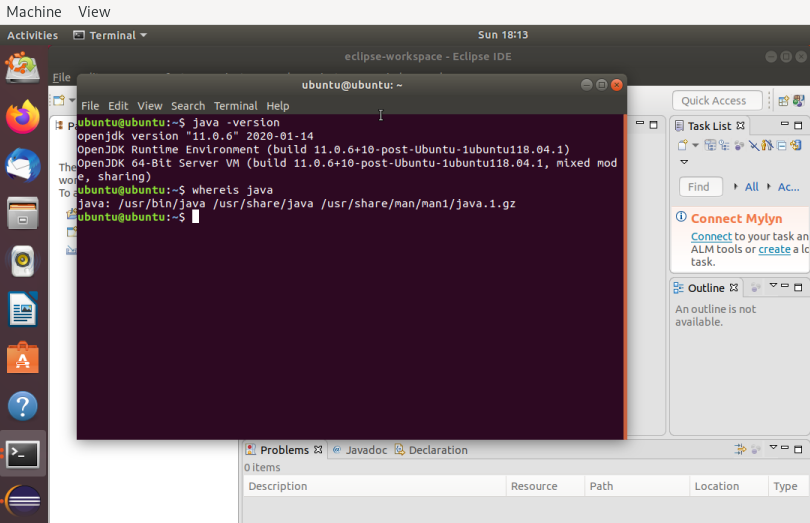
\includegraphics[width=\linewidth]{images/javaLive.png} 
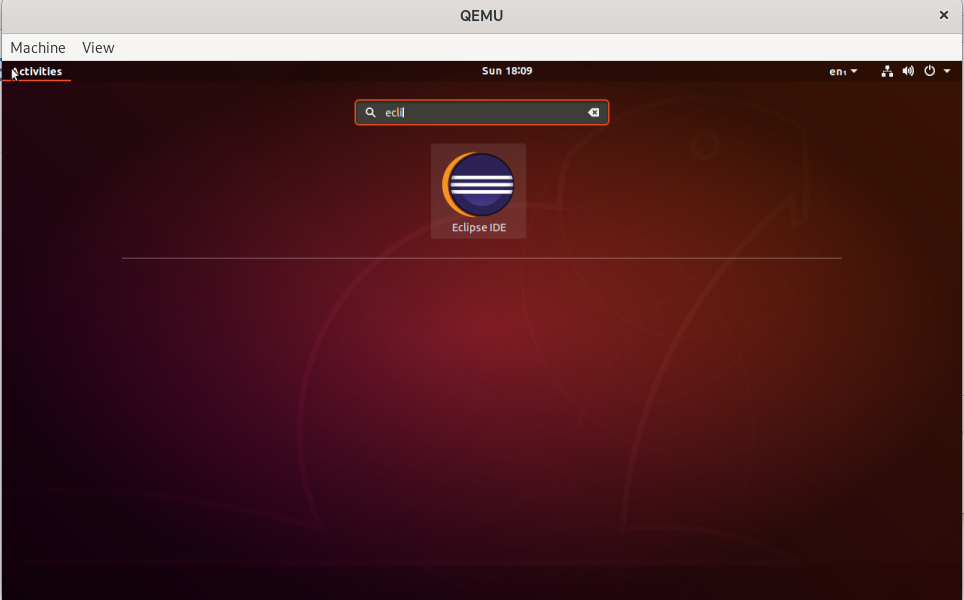
\includegraphics[width=\linewidth]{images/eclipseLive.png} 
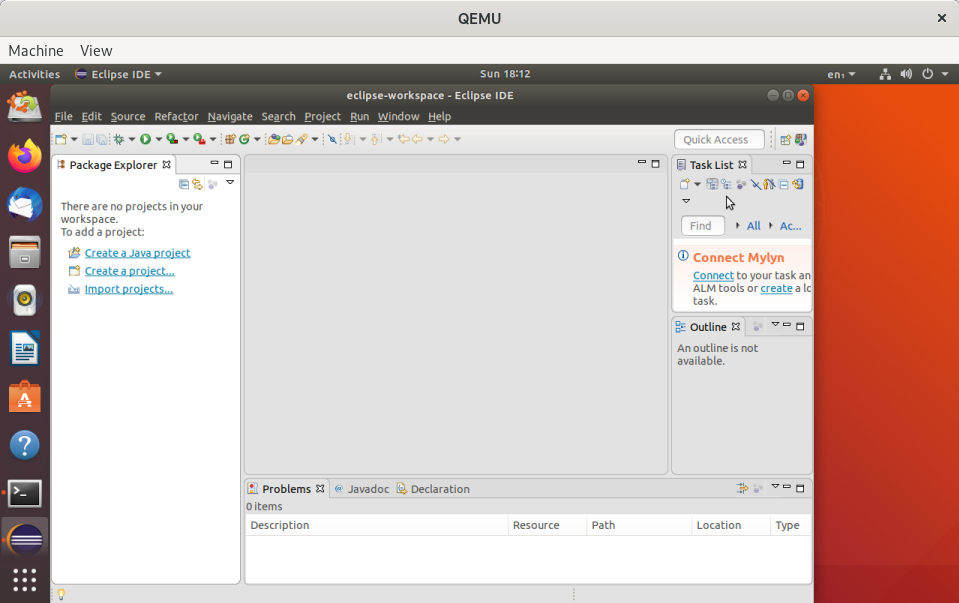
\includegraphics[width=\linewidth]{images/eclipseLive1.png} 

\chapter*{Modul Chrome}
\addcontentsline{toc}{chapter}{\numberline{}Modul Chrome}
Kao treci primjer modularizacije squashfs datotecnog sistema, kreiran je modul Chrome. Kao sto mu ime kaze, rijec je o modulu sa instaliranim Chrome pretrazivacem paketima. Vecinom koraci su identicni kao u prethodna 2 slucaja, izuzev koraka instaliranja dodatnih paketa unutar modula.\\
\begin{lstlisting}[style=BashInputStyle]
cd ~/squashfs/livecdtmp
sudo mount -o loop ./isoimgs/ubuntu-18.04.4-desktop-amd64.iso mnt
mkdir extract-chrome-cd
sudo rsync --exclude=/casper/filesystem.squashfs -a mnt/ extract-chrome-cd
mkdir modul-chrome
sudo rsync -a extract-chrome-cd/ modul-chrome
\end{lstlisting}
Zatim slijedi korak u kojem se opet raspakuje filesystem.squashfs direktorij i kopiramo ga u edit-chrome direktorij. Ovaj put cemo edit direktorij imenovati edit-chrome da ne izgubimo prethodni sadrzaj edit direktorija.\\
\begin{lstlisting}[style=BashInputStyle]
sudo unsquashfs mnt/casper/filesystem.squashfs
sudo mv squashfs-root/ edit-chrome
\end{lstlisting}

\noindent
Da bi imali mreznu konekciju unutar edit-chrome direktorija jedno rjesenje je kopirati /run direktorij unutar edit-chrome direktorija.
Najbolje manuelno popuniti resolv.conf unutar edit-chrome direktorija \\\textit{nameserver 1.1.1.1 \\
nameserver 8.8.8.8}.\\
Isto vazi i za etc/hosts datoteku. Najbolje je provjeriti nakon izvrsenih komandi da li je upisan sadrzaj u resolv.conf i hosts datoteke, te ukoliko nije dopuniti nedostatke:
\begin{lstlisting}[style=BashInputStyle]
sudo cp /etc/resolv.conf edit-chrome/etc/
sudo mount -o bind /run/ edit-chrome/run
\end{lstlisting}

\noindent
Kopirati i hosts direktorij/:
\begin{lstlisting}[style=BashInputStyle]
sudo cp /etc/hosts edit-chrome/etc/
\end{lstlisting}

\noindent
Namjestiti edit-chrome/dev direktorij kopirajuci /dev/ direktorij sa hosta, zatim chroot u edit-chrome direktorij.
Obaviti mount instrukcije navedene ispod. Ukoliko korisnik odluci da obrise edit-chrome direktorij iz nekog razloga,
bilo bi potrebno uraditi unmount edit-chrome direktorija da sistem domacin ne bi postao neupotrebljiv:
\begin{lstlisting}[style=BashInputStyle]
sudo mount --bind /dev/ edit-chrome/dev
sudo chroot edit-chrome
mount -t proc none /proc
mount -t sysfs none /sys
mount -t devpts none /dev/pts
\end{lstlisting}

\noindent
Takodjer potrebno je izvrsiti sljedece komande da bi se izbjegli problemi sa lokalizacijom:
\begin{lstlisting}[style=BashInputStyle]
export HOME=/root
export LC_ALL=C
\end{lstlisting}

\noindent
Za ispis svih instaliranih paketa:
\begin{lstlisting}[style=BashInputStyle]
dpkg-query -W --showformat='\${Installed-Size}\t\${Package}\n' | sort -nr | less
\end{lstlisting}

\noindent
Instalacija google-chrome paketa:
\begin{lstlisting}[style=BashInputStyle]
sudo nano /etc/apt/sources.list.d/google-chrome.list
\end{lstlisting}
Te upisati u ovu datoteku sljedeci sadrzaj
\begin{lstlisting}[style=BashInputStyle]
deb [arch=amd64] http://dl.google.com/linux/chrome/deb/ stable main
\end{lstlisting}
Zatim spasiti datoteku unutar nano editora sa \textbf{CTRL+O}, \textbf{ENTER} za potvrdu i \textbf{CTRL+X} za izlaz iz nano editora.\\
Sljedeca komanda preuzima Google javni kljuc da bismo mogli instalirati google-chrome. Zatim komandom apt-key dodajemo kljuc u prsten javnih kljuceva da bi apt mogao potvrditi integritet Google Chrome paketa.\\
\begin{lstlisting}[style=BashInputStyle]
wget https://dl.google.com/linux/linux_signing_key.pub
sudo apt-key add linux_signing_key.pub
\end{lstlisting}

Sada izvrsimo azuriranje liste paketa i instaliramo google-chrome-stable paket:
\begin{lstlisting}[style=BashInputStyle]
apt update
apt install google-chrome-stable
\end{lstlisting}

Provjera instalacije:
\begin{lstlisting}[style=BashInputStyle]
google-chrome-stable --version
\end{lstlisting}

\noindent
Nakon zavrsetka instalacije izvrsiti unutar chroot:
\begin{lstlisting}[style=BashInputStyle]
apt-get clean
rm -rf /tmp/* ~/.bash_history
rm -rf /tmp/* ~/.bashrc
rm /var/lib/dbus/machine-id
rm /sbin/initctl
dpkg-divert --rename --remove /sbin/initctl
umount /proc || umount -lf /proc
umount /sys
umount /dev/pts
exit
\end{lstlisting}

\noindent
Ponovno generisati filesystem.manifest:
\begin{lstlisting}[style=BashInputStyle]
sudo chmod +w extract-chrome-cd/casper/filesystem.manifest
sudo su
chroot edit-chrome dpkg-query -W --showformat='${Package} ${Version}\n' > extract-chrome-cd/casper/filesystem.manifest
exit
sudo cp extract-chrome-cd/casper/filesystem.manifest extract-chrome-cd/casper/filesystem.manifest-desktop
sudo sed -i '/ubiquity/d' extract-chrome-cd/casper/filesystem.manifest-desktop
sudo sed -i '/casper/d' extract-chrome-cd/casper/filesystem.manifest-desktop
sudo umount edit/dev
\end{lstlisting}

\noindent
Sada cemo upotrijebiti drugu funkciju iz squashfs-tools, a to je mksquashfs. S tom funkcijom cemo kompresovati edit-chrome direktorij u novu filesystem.squashfs datoteku. U kodu ispod je potrebno izvrsiti komandu iz linije 1 i jednu od preostale 3, pri cemu prva (komanda na liniji 2) daje najslabiju kompresiju, ali je najbrza. Druga komanda se duze izvrsava ali je veci procenat kompresije u odnosu na prvu komandu. Dok je kod trece komande procenat kompresije najveci, a vrijeme izvrsenja najduze:
\begin{lstlisting}[style=BashInputStyle]
sudo rm extract-chrome-cd/casper/filesystem.squashfs
sudo mksquashfs edit-chrome extract-chrome-cd/casper/filesystem.squashfs -nolzma 
sudo mksquashfs edit-chrome extract-chrome-cd/casper/filesystem.squashfs -b 1048576
sudo mksquashfs edit-chrome extract-chrome-cd/casper/filesystem.squashfs -comp xz -e edit/boot
\end{lstlisting}

\noindent
Naredni korak je da azuriramo filesystem.size datoteku:
\begin{lstlisting}[style=BashInputStyle]
sudo su
printf $(du -sx --block-size=1 edit-mysql | cut -f1) > extract-chrome-cd/casper/filesystem.size
exit
\end{lstlisting}

\noindent
Nakon toga upisati naziv image-a unutar README.diskdefines. 
Upisati 'Ubuntu with Google Chrome 18.04.4 LTS "Bionic Beaver" - Release amd64' u polje DISKNAME:
\begin{lstlisting}[style=BashInputStyle]
sudo gedit extract-chrome-cd/README.diskdefines
\end{lstlisting}

\noindent
Azurirati md5sum.txt datoteku:
\begin{lstlisting}[style=BashInputStyle]
cd extract-chrome-cd
sudo rm md5sum.txt
find -type f -print0 | sudo xargs -0 md5sum | grep -v isolinux/boot.cat | sudo tee md5sum.txt
\end{lstlisting}

\noindent
Napokon mozemo napraviti iso image koji ce da sadrzi Google Chrome modul. Za ovu operaciju koristimo funkciju genisoimage. Neke linux distribucije nude mkisofs funkciju. Tako da ukoliko ne radi genisoimage trebala bi raditi funkcija mkisofs:
\begin{lstlisting}[style=BashInputStyle]
sudo genisoimage -D -r -V "$IMAGE_NAME" -cache-inodes -J -l -b isolinux/isolinux.bin -c isolinux/boot.cat -no-emul-boot -boot-load-size 4 -boot-info-table -o ../ubuntu-with-chrome-18.04-amd64.iso .
\end{lstlisting}

\noindent
Sada cemo napraviti virtuelni hard disk pomocu qemu-img komande da bismo pokrenuli na njemu nas novi modul Google Chrome Ubuntu.
\begin{lstlisting}[style=BashInputStyle]
cd ~
qemu-img create ubuntuchrome.img 5G
\end{lstlisting}

\noindent 
Pokrenucemo modul pomocu KVM-a:
\begin{lstlisting}[style=BashInputStyle]
sudo kvm -hda ubuntuchrome.img -cdrom ~/zavrsni/livecdtmp/ubuntu-with-chrome-18.04-amd64.iso -boot d -m 2048
\end{lstlisting}

%\subsection*{Rezultat Modul Chrome}
%\addcontentsline{toc}{subsection}{\numberline{}Rezultat Modul Chrome}
%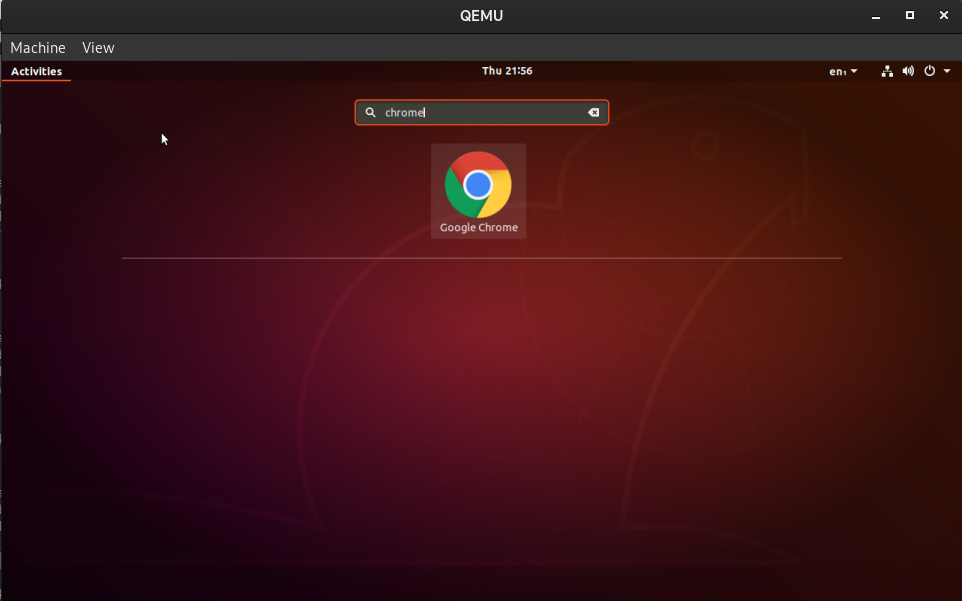
\includegraphics[width=\linewidth]{images/chromeLive.png} 


\end{document}
